\documentclass[]{article}
\usepackage{lmodern}
\usepackage{amssymb,amsmath}
\usepackage{ifxetex,ifluatex}
\usepackage{fixltx2e} % provides \textsubscript
\ifnum 0\ifxetex 1\fi\ifluatex 1\fi=0 % if pdftex
  \usepackage[T1]{fontenc}
  \usepackage[utf8]{inputenc}
\else % if luatex or xelatex
  \ifxetex
    \usepackage{mathspec}
  \else
    \usepackage{fontspec}
  \fi
  \defaultfontfeatures{Ligatures=TeX,Scale=MatchLowercase}
\fi
% use upquote if available, for straight quotes in verbatim environments
\IfFileExists{upquote.sty}{\usepackage{upquote}}{}
% use microtype if available
\IfFileExists{microtype.sty}{%
\usepackage{microtype}
\UseMicrotypeSet[protrusion]{basicmath} % disable protrusion for tt fonts
}{}
\usepackage[margin=1in]{geometry}
\usepackage{hyperref}
\hypersetup{unicode=true,
            pdftitle={Steven Maharaj 695281 Assignment 2, Question 2},
            pdfborder={0 0 0},
            breaklinks=true}
\urlstyle{same}  % don't use monospace font for urls
\usepackage{color}
\usepackage{fancyvrb}
\newcommand{\VerbBar}{|}
\newcommand{\VERB}{\Verb[commandchars=\\\{\}]}
\DefineVerbatimEnvironment{Highlighting}{Verbatim}{commandchars=\\\{\}}
% Add ',fontsize=\small' for more characters per line
\usepackage{framed}
\definecolor{shadecolor}{RGB}{248,248,248}
\newenvironment{Shaded}{\begin{snugshade}}{\end{snugshade}}
\newcommand{\KeywordTok}[1]{\textcolor[rgb]{0.13,0.29,0.53}{\textbf{#1}}}
\newcommand{\DataTypeTok}[1]{\textcolor[rgb]{0.13,0.29,0.53}{#1}}
\newcommand{\DecValTok}[1]{\textcolor[rgb]{0.00,0.00,0.81}{#1}}
\newcommand{\BaseNTok}[1]{\textcolor[rgb]{0.00,0.00,0.81}{#1}}
\newcommand{\FloatTok}[1]{\textcolor[rgb]{0.00,0.00,0.81}{#1}}
\newcommand{\ConstantTok}[1]{\textcolor[rgb]{0.00,0.00,0.00}{#1}}
\newcommand{\CharTok}[1]{\textcolor[rgb]{0.31,0.60,0.02}{#1}}
\newcommand{\SpecialCharTok}[1]{\textcolor[rgb]{0.00,0.00,0.00}{#1}}
\newcommand{\StringTok}[1]{\textcolor[rgb]{0.31,0.60,0.02}{#1}}
\newcommand{\VerbatimStringTok}[1]{\textcolor[rgb]{0.31,0.60,0.02}{#1}}
\newcommand{\SpecialStringTok}[1]{\textcolor[rgb]{0.31,0.60,0.02}{#1}}
\newcommand{\ImportTok}[1]{#1}
\newcommand{\CommentTok}[1]{\textcolor[rgb]{0.56,0.35,0.01}{\textit{#1}}}
\newcommand{\DocumentationTok}[1]{\textcolor[rgb]{0.56,0.35,0.01}{\textbf{\textit{#1}}}}
\newcommand{\AnnotationTok}[1]{\textcolor[rgb]{0.56,0.35,0.01}{\textbf{\textit{#1}}}}
\newcommand{\CommentVarTok}[1]{\textcolor[rgb]{0.56,0.35,0.01}{\textbf{\textit{#1}}}}
\newcommand{\OtherTok}[1]{\textcolor[rgb]{0.56,0.35,0.01}{#1}}
\newcommand{\FunctionTok}[1]{\textcolor[rgb]{0.00,0.00,0.00}{#1}}
\newcommand{\VariableTok}[1]{\textcolor[rgb]{0.00,0.00,0.00}{#1}}
\newcommand{\ControlFlowTok}[1]{\textcolor[rgb]{0.13,0.29,0.53}{\textbf{#1}}}
\newcommand{\OperatorTok}[1]{\textcolor[rgb]{0.81,0.36,0.00}{\textbf{#1}}}
\newcommand{\BuiltInTok}[1]{#1}
\newcommand{\ExtensionTok}[1]{#1}
\newcommand{\PreprocessorTok}[1]{\textcolor[rgb]{0.56,0.35,0.01}{\textit{#1}}}
\newcommand{\AttributeTok}[1]{\textcolor[rgb]{0.77,0.63,0.00}{#1}}
\newcommand{\RegionMarkerTok}[1]{#1}
\newcommand{\InformationTok}[1]{\textcolor[rgb]{0.56,0.35,0.01}{\textbf{\textit{#1}}}}
\newcommand{\WarningTok}[1]{\textcolor[rgb]{0.56,0.35,0.01}{\textbf{\textit{#1}}}}
\newcommand{\AlertTok}[1]{\textcolor[rgb]{0.94,0.16,0.16}{#1}}
\newcommand{\ErrorTok}[1]{\textcolor[rgb]{0.64,0.00,0.00}{\textbf{#1}}}
\newcommand{\NormalTok}[1]{#1}
\usepackage{longtable,booktabs}
\usepackage{graphicx,grffile}
\makeatletter
\def\maxwidth{\ifdim\Gin@nat@width>\linewidth\linewidth\else\Gin@nat@width\fi}
\def\maxheight{\ifdim\Gin@nat@height>\textheight\textheight\else\Gin@nat@height\fi}
\makeatother
% Scale images if necessary, so that they will not overflow the page
% margins by default, and it is still possible to overwrite the defaults
% using explicit options in \includegraphics[width, height, ...]{}
\setkeys{Gin}{width=\maxwidth,height=\maxheight,keepaspectratio}
\IfFileExists{parskip.sty}{%
\usepackage{parskip}
}{% else
\setlength{\parindent}{0pt}
\setlength{\parskip}{6pt plus 2pt minus 1pt}
}
\setlength{\emergencystretch}{3em}  % prevent overfull lines
\providecommand{\tightlist}{%
  \setlength{\itemsep}{0pt}\setlength{\parskip}{0pt}}
\setcounter{secnumdepth}{0}
% Redefines (sub)paragraphs to behave more like sections
\ifx\paragraph\undefined\else
\let\oldparagraph\paragraph
\renewcommand{\paragraph}[1]{\oldparagraph{#1}\mbox{}}
\fi
\ifx\subparagraph\undefined\else
\let\oldsubparagraph\subparagraph
\renewcommand{\subparagraph}[1]{\oldsubparagraph{#1}\mbox{}}
\fi

%%% Use protect on footnotes to avoid problems with footnotes in titles
\let\rmarkdownfootnote\footnote%
\def\footnote{\protect\rmarkdownfootnote}

%%% Change title format to be more compact
\usepackage{titling}

% Create subtitle command for use in maketitle
\providecommand{\subtitle}[1]{
  \posttitle{
    \begin{center}\large#1\end{center}
    }
}

\setlength{\droptitle}{-2em}

  \title{Steven Maharaj 695281 Assignment 2, Question 2}
    \pretitle{\vspace{\droptitle}\centering\huge}
  \posttitle{\par}
    \author{}
    \preauthor{}\postauthor{}
    \date{}
    \predate{}\postdate{}
  
\usepackage{bm}
\usepackage{amsmath}
\usepackage{amsfonts}
\usepackage{amssymb}

\begin{document}
\maketitle

\textbf{Due: Friday 20 September 2019}\\
\vspace{5 mm}

\textbf{There are places in this assignment where R code will be
required. Therefore set the random seed so assignment is reproducible.}

\begin{Shaded}
\begin{Highlighting}[]
\KeywordTok{set.seed}\NormalTok{(}\DecValTok{695281}\NormalTok{) }\CommentTok{#Please change random seed to your student id number.}
\KeywordTok{library}\NormalTok{(dplyr)}
\end{Highlighting}
\end{Shaded}

\begin{verbatim}
## 
## Attaching package: 'dplyr'
\end{verbatim}

\begin{verbatim}
## The following objects are masked from 'package:stats':
## 
##     filter, lag
\end{verbatim}

\begin{verbatim}
## The following objects are masked from 'package:base':
## 
##     intersect, setdiff, setequal, union
\end{verbatim}

\begin{Shaded}
\begin{Highlighting}[]
\KeywordTok{library}\NormalTok{(mvtnorm)}
\KeywordTok{library}\NormalTok{(coda)}
\end{Highlighting}
\end{Shaded}

PART A

\begin{Shaded}
\begin{Highlighting}[]
\CommentTok{# Read the Data}
\NormalTok{Hiron <-}\StringTok{ }\KeywordTok{read.csv}\NormalTok{(}\StringTok{"Hiron.csv"}\NormalTok{)}
\NormalTok{HironHomo <-}\StringTok{ }\NormalTok{Hiron }\OperatorTok\KeywordTok{filter}\NormalTok{(homc282y}\OperatorTok{==}\DecValTok{1}\NormalTok{) }\OperatorTok\StringTok{ }\KeywordTok{select}\NormalTok{(}\OperatorTok{-}\NormalTok{idnum)}
\NormalTok{Hiron <-}\StringTok{ }\KeywordTok{read.csv}\NormalTok{(}\StringTok{"Hiron.csv"}\NormalTok{)}
\NormalTok{HironWild <-}\StringTok{ }\NormalTok{Hiron }\OperatorTok\KeywordTok{filter}\NormalTok{(homc282y}\OperatorTok{==}\DecValTok{0}\NormalTok{) }\OperatorTok\StringTok{ }\KeywordTok{select}\NormalTok{(}\OperatorTok{-}\NormalTok{idnum)}
\end{Highlighting}
\end{Shaded}

\begin{Shaded}
\begin{Highlighting}[]
\CommentTok{#fit linear regression using lm}

\NormalTok{model <-}\StringTok{ }\KeywordTok{lm}\NormalTok{(logsf }\OperatorTok{~}\StringTok{ }\NormalTok{time,}\DataTypeTok{data =}\NormalTok{ HironHomo)}
\NormalTok{model}\OperatorTok{$}\NormalTok{coefficients}
\end{Highlighting}
\end{Shaded}

\begin{verbatim}
## (Intercept)        time 
##  4.23987253  0.07126085
\end{verbatim}

\begin{Shaded}
\begin{Highlighting}[]
\NormalTok{intercept <-}\KeywordTok{matrix}\NormalTok{(}\DecValTok{1}\NormalTok{,}\KeywordTok{length}\NormalTok{(HironHomo}\OperatorTok{$}\NormalTok{time),}\DecValTok{1}\NormalTok{)}

\NormalTok{X <-}\StringTok{ }\KeywordTok{cbind}\NormalTok{(intercept,HironHomo}\OperatorTok{$}\NormalTok{time)}
\NormalTok{XTX <-}\StringTok{ }\KeywordTok{crossprod}\NormalTok{(X)  }
\NormalTok{XTXinv <-}\KeywordTok{solve}\NormalTok{(XTX)}
\CommentTok{# (XTX)^-1}
\NormalTok{XTXinv}
\end{Highlighting}
\end{Shaded}

\begin{verbatim}
##              [,1]          [,2]
## [1,]  0.033734956 -0.0015415009
## [2,] -0.001541501  0.0001062175
\end{verbatim}

\begin{Shaded}
\begin{Highlighting}[]
\CommentTok{#Estimated error variance}
\NormalTok{Sigma2<-}\KeywordTok{sigma}\NormalTok{(model)}\OperatorTok{^}\DecValTok{2}
\NormalTok{Sigma2}
\end{Highlighting}
\end{Shaded}

\begin{verbatim}
## [1] 1.715042
\end{verbatim}

\begin{longtable}[]{@{}l@{}}
\toprule
\begin{minipage}[t]{0.97\columnwidth}\raggedright\strut
PART B\strut
\end{minipage}\tabularnewline
\begin{minipage}[t]{0.97\columnwidth}\raggedright\strut
Define the Gibbs sampler function\strut
\end{minipage}\tabularnewline
\begin{minipage}[t]{0.97\columnwidth}\raggedright\strut
```r \#This is a Gibbs sampler where beta is updated as a block. The
arguments are \#X: matrix of predictors dimension n times p.~Includes
the intercept. \#y: response vector, length p. \#tau0: initial value for
the residual precision. \#iter: number of iterations \#burnin: number of
initial iterations to remove
Gibbs.lm1\textless{}-function(X,y,tau0,iter,burnin)\{ p \textless{}-
dim(X){[}2{]} \#number of predictors\strut
\end{minipage}\tabularnewline
\begin{minipage}[t]{0.97\columnwidth}\raggedright\strut
\# X \textless{}- as.numeric(X) \# y \textless{}- as.numeric(y) XTX
\textless{}- crossprod(X) XTXinv \textless{}-solve(XTX) XTY \textless{}-
crossprod(X,y) betahat\textless{}-solve(XTX,XTY) \#betahat =
(t(X)\%\emph{\%X)\^{}\{-1\}t(X)\%}\%y = mean of conditional posterior
for beta tau \textless{}-tau0 T\_rep \textless{}- rep(0,iter) T\_y
\textless{}- rep(0,iter) library(mvtnorm)\strut
\end{minipage}\tabularnewline
\begin{minipage}[t]{0.97\columnwidth}\raggedright\strut
par\textless{}-matrix(0,iter,p+1) \#storing iterations, beta (length p)
+ tau (length 1) for( i in 1:iter)\{ beta \textless{}-
rmvnorm(1,mean=betahat,sigma=XTXinv/tau) \#sample beta beta \textless{}-
as.numeric(beta) err \textless{}- y-X\%\emph{\%beta tau \textless{}-
rgamma(1,0.5}n,0.5*sum(err\^{}2)) \#sample tau. par{[}i,{]}
\textless{}-c(beta,tau) \#store current round of beta, tau in par.\strut
\end{minipage}\tabularnewline
\begin{minipage}[t]{0.97\columnwidth}\raggedright\strut
\# posterior checking Xbeta\_rep \textless{}- X\%\emph{\%as.vector(beta)
y\_rep \textless{}- Xbeta\_rep+rnorm(length(y))}sqrt(1/tau) err\_rep
\textless{}- y\_rep-Xbeta\_rep\strut
\end{minipage}\tabularnewline
\begin{minipage}[t]{0.97\columnwidth}\raggedright\strut
T\_rep{[}i{]} \textless{}- sum(err\_rep\^{}2) T\_y{[}i{]} \textless{}-
sum(err\^{}2) \} print(``Performing posterior predictive checking we
have a p value'') pval \textless{}-
prop.table(table(T\_rep\textgreater{}T\_y)){[}``TRUE''{]} print(pval)
par \textless{}-par{[}-c(1:burnin),{]} \#removing the first iterations
par{[},3{]} \textless{}- 1/par{[},3{]} colnames(par) \textless{}-
c(`beta0',`beta1',`sigma2') return(par) \} ```\strut
\end{minipage}\tabularnewline
\begin{minipage}[t]{0.97\columnwidth}\raggedright\strut
```r data\textless{}-HironWild response \textless{}-
data\(logsf #response variable n<-dim(data)[1] intercept <-matrix(1,n,1) #Intercept (to be estimated without penalty) X <- cbind(intercept,data\)time)\strut
\end{minipage}\tabularnewline
\begin{minipage}[t]{0.97\columnwidth}\raggedright\strut
\# run two chains
system.time(chain1\textless{}-Gibbs.lm1(X=X,y=response,tau0=1/Sigma2,iter=10000,burnin=1000))
```\strut
\end{minipage}\tabularnewline
\begin{minipage}[t]{0.97\columnwidth}\raggedright\strut
\texttt{\#\#\ {[}1{]}\ "Performing\ posterior\ predictive\ checking\ we\ have\ a\ p\ value"\ \#\#\ \ \ TRUE\ \#\#\ 0.5067}\strut
\end{minipage}\tabularnewline
\begin{minipage}[t]{0.97\columnwidth}\raggedright\strut
\texttt{\#\#\ \ \ \ user\ \ system\ elapsed\ \#\#\ \ \ 1.722\ \ \ 0.012\ \ \ 1.744}\strut
\end{minipage}\tabularnewline
\begin{minipage}[t]{0.97\columnwidth}\raggedright\strut
\texttt{r\ system.time(chain2\textless{}-Gibbs.lm1(X=X,y=response,tau0=1/Sigma2,iter=10000,burnin=1000))}\strut
\end{minipage}\tabularnewline
\begin{minipage}[t]{0.97\columnwidth}\raggedright\strut
\texttt{\#\#\ {[}1{]}\ "Performing\ posterior\ predictive\ checking\ we\ have\ a\ p\ value"\ \#\#\ \ \ TRUE\ \#\#\ 0.4992}\strut
\end{minipage}\tabularnewline
\begin{minipage}[t]{0.97\columnwidth}\raggedright\strut
\texttt{\#\#\ \ \ \ user\ \ system\ elapsed\ \#\#\ \ \ 1.671\ \ \ 0.005\ \ \ 1.676}\strut
\end{minipage}\tabularnewline
\begin{minipage}[t]{0.97\columnwidth}\raggedright\strut
```r \# Remove every second iteration to reduce auto - corrlation\strut
\end{minipage}\tabularnewline
\begin{minipage}[t]{0.97\columnwidth}\raggedright\strut
chain1 \textless{}- chain1{[}seq(1,dim(chain1){[}1{]},by=2),{]} chain2
\textless{}- chain2{[}seq(1,dim(chain2){[}1{]},by=2),{]} ```\strut
\end{minipage}\tabularnewline
\begin{minipage}[t]{0.97\columnwidth}\raggedright\strut
```r chain12 \textless{}- rbind(chain1,chain2) chain\_stats \textless{}-
data.frame(matrix(nrow = 3,ncol =4 )) para\_names \textless{}-
c(`beta0',`beta1',`sigma2',`lower\_CI95',`upper\_CI95') for (i in 1:3)
\{ chain \textless{}- chain12{[},i{]} quat \textless{}-
quantile(sort(chain), c(0.05, 0.975)) chain\_stats{[}i,{]} \textless{}-
c(mean(chain),sd(chain),quat) \} names(chain\_stats)\textless{}-
c(``posterior mean'',``std'',`lower\_CI95',`upper\_CI95')\strut
\end{minipage}\tabularnewline
\begin{minipage}[t]{0.97\columnwidth}\raggedright\strut
row.names(chain\_stats) \textless{}- c(`beta0',`beta1',`sigma2')\strut
\end{minipage}\tabularnewline
\begin{minipage}[t]{0.97\columnwidth}\raggedright\strut
\# chain results chain\_stats ```\strut
\end{minipage}\tabularnewline
\begin{minipage}[t]{0.97\columnwidth}\raggedright\strut
\texttt{\#\#\ \ \ \ \ \ \ \ posterior\ mean\ \ \ \ \ \ \ \ \ std\ lower\_CI95\ upper\_CI95\ \#\#\ beta0\ \ \ \ \ \ 4.02321818\ 0.105666806\ 3.84913355\ 4.23109147\ \#\#\ beta1\ \ \ \ \ \ 0.02016437\ 0.005384182\ 0.01130925\ 0.03055483\ \#\#\ sigma2\ \ \ \ \ 0.87362582\ 0.080795467\ 0.74950070\ 1.04659356}\strut
\end{minipage}\tabularnewline
\bottomrule
\end{longtable}

PART C

\begin{Shaded}
\begin{Highlighting}[]
\CommentTok{# beta0}


\KeywordTok{plot}\NormalTok{(chain1[,}\DecValTok{1}\NormalTok{],}\DataTypeTok{type=}\StringTok{'l'}\NormalTok{,}\DataTypeTok{ylab=}\KeywordTok{expression}\NormalTok{(beta[}\DecValTok{0}\NormalTok{]))}
\KeywordTok{lines}\NormalTok{(chain1[,}\DecValTok{1}\NormalTok{],}\DataTypeTok{type=}\StringTok{'l'}\NormalTok{,}\DataTypeTok{col=}\DecValTok{1}\NormalTok{,}\DataTypeTok{ylab=}\KeywordTok{expression}\NormalTok{(beta[}\DecValTok{0}\NormalTok{]))}
\KeywordTok{lines}\NormalTok{(chain2[,}\DecValTok{1}\NormalTok{],}\DataTypeTok{type=}\StringTok{'l'}\NormalTok{,}\DataTypeTok{col=}\DecValTok{2}\NormalTok{,}\DataTypeTok{ylab=}\KeywordTok{expression}\NormalTok{(beta[}\DecValTok{0}\NormalTok{]))}
\KeywordTok{legend}\NormalTok{(}\StringTok{'topright'}\NormalTok{,}\DataTypeTok{legend=}\KeywordTok{c}\NormalTok{(}\StringTok{'Chain 1'}\NormalTok{,}\StringTok{'Chain 2'}\NormalTok{),}\DataTypeTok{col=}\DecValTok{1}\OperatorTok{:}\DecValTok{2}\NormalTok{,}\DataTypeTok{lty=}\DecValTok{1}\NormalTok{,}\DataTypeTok{bty=}\StringTok{'n'}\NormalTok{)}
\end{Highlighting}
\end{Shaded}

\includegraphics{Q2_files/figure-latex/unnamed-chunk-7-1.pdf}

\begin{Shaded}
\begin{Highlighting}[]
\CommentTok{# beta1}
\KeywordTok{plot}\NormalTok{(chain1[,}\DecValTok{2}\NormalTok{],}\DataTypeTok{type=}\StringTok{'l'}\NormalTok{,}\DataTypeTok{ylab=}\KeywordTok{expression}\NormalTok{(beta[}\DecValTok{1}\NormalTok{]))}
\KeywordTok{lines}\NormalTok{(chain1[,}\DecValTok{2}\NormalTok{],}\DataTypeTok{type=}\StringTok{'l'}\NormalTok{,}\DataTypeTok{col=}\DecValTok{1}\NormalTok{,}\DataTypeTok{ylab=}\KeywordTok{expression}\NormalTok{(beta[}\DecValTok{1}\NormalTok{]))}
\KeywordTok{lines}\NormalTok{(chain2[,}\DecValTok{2}\NormalTok{],}\DataTypeTok{type=}\StringTok{'l'}\NormalTok{,}\DataTypeTok{col=}\DecValTok{2}\NormalTok{,}\DataTypeTok{ylab=}\KeywordTok{expression}\NormalTok{(beta[}\DecValTok{1}\NormalTok{]))}
\KeywordTok{legend}\NormalTok{(}\StringTok{'topright'}\NormalTok{,}\DataTypeTok{legend=}\KeywordTok{c}\NormalTok{(}\StringTok{'Chain 1'}\NormalTok{,}\StringTok{'Chain 2'}\NormalTok{),}\DataTypeTok{col=}\DecValTok{1}\OperatorTok{:}\DecValTok{2}\NormalTok{,}\DataTypeTok{lty=}\DecValTok{1}\NormalTok{,}\DataTypeTok{bty=}\StringTok{'n'}\NormalTok{) }
\end{Highlighting}
\end{Shaded}

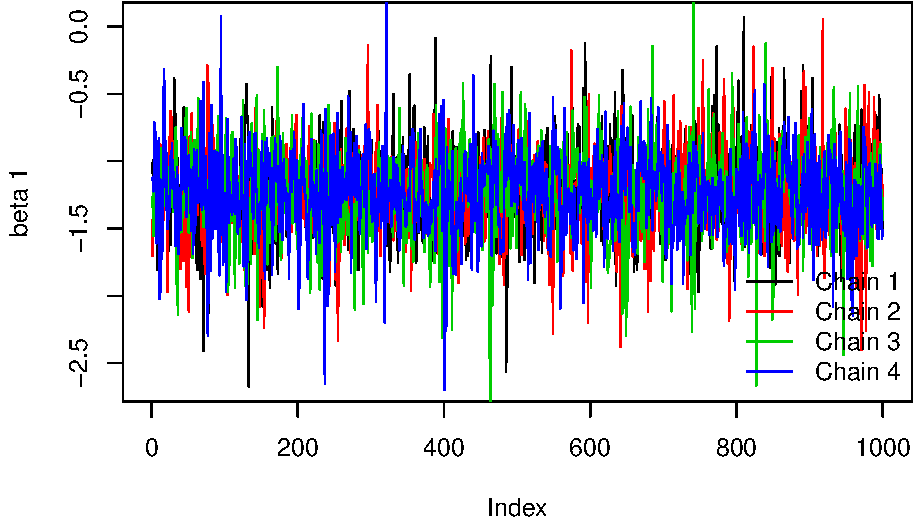
\includegraphics{Q2_files/figure-latex/unnamed-chunk-8-1.pdf}

\begin{Shaded}
\begin{Highlighting}[]
\CommentTok{# sigma^2}
\KeywordTok{plot}\NormalTok{(chain1[,}\DecValTok{3}\NormalTok{],}\DataTypeTok{type=}\StringTok{'l'}\NormalTok{,}\DataTypeTok{ylab=}\KeywordTok{expression}\NormalTok{(sigma}\OperatorTok{^}\DecValTok{2}\NormalTok{))}
\KeywordTok{lines}\NormalTok{(chain1[,}\DecValTok{3}\NormalTok{],}\DataTypeTok{type=}\StringTok{'l'}\NormalTok{,}\DataTypeTok{col=}\DecValTok{1}\NormalTok{,}\DataTypeTok{ylab=}\KeywordTok{expression}\NormalTok{(sigma}\OperatorTok{^}\DecValTok{2}\NormalTok{))}
\KeywordTok{lines}\NormalTok{(chain2[,}\DecValTok{3}\NormalTok{],}\DataTypeTok{type=}\StringTok{'l'}\NormalTok{,}\DataTypeTok{col=}\DecValTok{2}\NormalTok{,}\DataTypeTok{ylab=}\KeywordTok{expression}\NormalTok{(sigma}\OperatorTok{^}\DecValTok{2}\NormalTok{))}
\KeywordTok{legend}\NormalTok{(}\StringTok{'topright'}\NormalTok{,}\DataTypeTok{legend=}\KeywordTok{c}\NormalTok{(}\StringTok{'Chain 1'}\NormalTok{,}\StringTok{'Chain 2'}\NormalTok{),}\DataTypeTok{col=}\DecValTok{1}\OperatorTok{:}\DecValTok{2}\NormalTok{,}\DataTypeTok{lty=}\DecValTok{1}\NormalTok{,}\DataTypeTok{bty=}\StringTok{'n'}\NormalTok{) }
\end{Highlighting}
\end{Shaded}

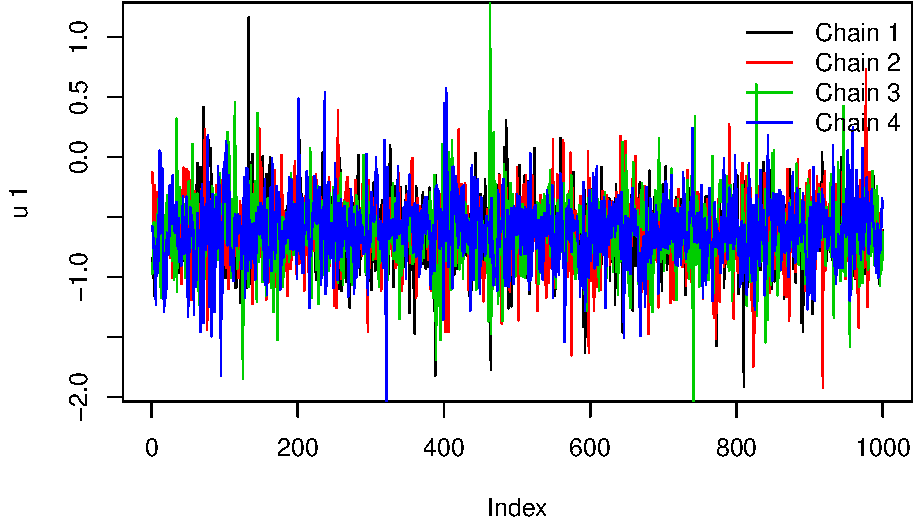
\includegraphics{Q2_files/figure-latex/unnamed-chunk-9-1.pdf}

\begin{Shaded}
\begin{Highlighting}[]
\CommentTok{#Gelman-Rubin diagnostic}

\NormalTok{chains <-}\StringTok{ }\KeywordTok{mcmc.list}\NormalTok{(}\KeywordTok{mcmc}\NormalTok{(chain1),}\KeywordTok{mcmc}\NormalTok{(chain2))}
\KeywordTok{gelman.diag}\NormalTok{(chains)[[}\DecValTok{1}\NormalTok{]]}
\end{Highlighting}
\end{Shaded}

\begin{verbatim}
##        Point est. Upper C.I.
## beta0   1.0002329  1.0003600
## beta1   0.9998113  0.9998467
## sigma2  1.0012570  1.0065257
\end{verbatim}

\begin{center}\rule{0.5\linewidth}{\linethickness}\end{center}

PART D

\begin{Shaded}
\begin{Highlighting}[]
\CommentTok{# Fit regresssion for all of the data}

\NormalTok{full_model <-}\StringTok{ }\KeywordTok{lm}\NormalTok{(logsf }\OperatorTok{~}\StringTok{ }\NormalTok{time,}\DataTypeTok{data =}\NormalTok{ Hiron)}
\KeywordTok{summary}\NormalTok{(full_model)}
\end{Highlighting}
\end{Shaded}

\begin{verbatim}
## 
## Call:
## lm(formula = logsf ~ time, data = Hiron)
## 
## Residuals:
##     Min      1Q  Median      3Q     Max 
## -3.5197 -0.6597  0.0770  0.7523  2.6978 
## 
## Coefficients:
##             Estimate Std. Error t value Pr(>|t|)    
## (Intercept) 4.130162   0.110870  37.252  < 2e-16 ***
## time        0.029599   0.005769   5.131 4.95e-07 ***
## ---
## Signif. codes:  0 '***' 0.001 '**' 0.01 '*' 0.05 '.' 0.1 ' ' 1
## 
## Residual standard error: 1.152 on 328 degrees of freedom
## Multiple R-squared:  0.07429,    Adjusted R-squared:  0.07147 
## F-statistic: 26.32 on 1 and 328 DF,  p-value: 4.952e-07
\end{verbatim}

\begin{Shaded}
\begin{Highlighting}[]
\CommentTok{# Estimates}
\NormalTok{full_model}\OperatorTok{$}\NormalTok{coefficients}
\end{Highlighting}
\end{Shaded}

\begin{verbatim}
## (Intercept)        time 
##  4.13016198  0.02959941
\end{verbatim}

\begin{Shaded}
\begin{Highlighting}[]
\CommentTok{# 95 % confidence intervals}
\KeywordTok{confint}\NormalTok{(full_model)}
\end{Highlighting}
\end{Shaded}

\begin{verbatim}
##                  2.5 %     97.5 %
## (Intercept) 3.91205524 4.34826873
## time        0.01825025 0.04094857
\end{verbatim}


\end{document}
